\documentclass[10pt,a4paper,twoside, twocolumn]{report}
%% Lots of packages !
\usepackage{etex}

%% Francisation
\usepackage[francais]{babel}
\usepackage[T1]{fontenc}
\usepackage[utf8]{inputenc}
%\usepackage{textcomp}

%% Réglages généraux
\usepackage[left=1.5cm,right=1.5cm,top=2cm,bottom=2cm]{geometry}
\usepackage{fancyhdr}
\usepackage{setspace}
\usepackage{lscape}
%\usepackage{multicol}
\usepackage{makeidx}
\usepackage[clearempty]{titlesec}
\usepackage{cite}

%% Packages pour le texte
\usepackage{pifont}
\usepackage{eurosym}
\usepackage{soul}
\usepackage[normalem]{ulem}
\usepackage{fancybox}
\usepackage{boxedminipage}
\usepackage{enumerate}
\usepackage{verbatim}
\usepackage{moreverb}
\usepackage{listings}
\usepackage[table]{xcolor}

%% Packages pour les tableaux
\usepackage{array}
\usepackage{multirow}
\usepackage{tabularx}
\usepackage{longtable}

%% Packages pour les dessins
\usepackage{graphicx}
\usepackage{wrapfig}
%\usepackage{picins}
\usepackage{picinpar}
\usepackage{epic}
\usepackage{eepic}
\usepackage{tikz}
\usepackage{afterpage}
\usepackage{rotating}
\usepackage{float}
\usepackage{caption}

%% Packages pour les maths
\usepackage{amsmath}
\usepackage{amssymb}
\usepackage{dsfont}
\usepackage{mathrsfs}
\usepackage{bussproofs}
\usepackage[thmmarks,amsmath]{ntheorem}

%% Création de nouvelles commandes
%\usepackage{calc}
\usepackage{ifthen}
\usepackage{xspace}



\usepackage{url}
\usepackage{hyperref}
\usepackage{todonotes}
\usepackage{subcaption}
\usepackage[french,ruled,vlined,linesnumbered,algochapter,dotocloa]{algorithm2e}
\usepackage{MnSymbol}

\usepackage{chngcntr}

\usepackage{standalone}
\usepackage{import}



\frenchbsetup{StandardEnumerateEnv=true}

%% =======================================================================

\fancypagestyle{empty}{%
  \fancyhf{}
  \fancyhead[L]{}
  \fancyhead[C]{}
  \fancyhead[R]{}
  \fancyfoot[L]{}
  \fancyfoot[C]{}
  \fancyfoot[R]{}
}
\fancypagestyle{basicstyle}{
	\fancyhf{}	
	\fancyhead[L]{}
	\fancyhead[C]{Rendu réaliste et temps réel pour la réalité augmentée}
	\fancyhead[R]{}
	\fancyfoot[L]{hadrien.croubois@ens-lyon.fr}
	\fancyfoot[C]{--~\thepage~--}
	\fancyfoot[R]{}
}
\pagestyle{basicstyle}

%% =======================================================================

\titleformat{\section}[frame]
{\normalfont}
{\filright \footnotesize \enspace Partie \thesection\enspace}
{6pt}
{\bfseries\filcenter}
	
\titleformat{\subsection}[frame]
{\normalfont}
{\filright \footnotesize \enspace \thesubsection\enspace}
{6pt}
{\filcenter}

\titleformat{\subsubsection}
{\titlerule \vspace{.8ex} \normalfont\itshape}
{\thesubsubsection}
{.5em}
{}

\titleformat{\chapter}[display]
{\normalfont\bfseries\filcenter}
{}
{1ex}
{\titlerule[2pt] \vspace{2ex} \LARGE}
[\vspace{1ex} {\titlerule[2pt]}]

\parindent=10pt
\DeclareUnicodeCharacter{00A0}{~}

%% =======================================================================



\newcommand{\HRule}{\rule{\linewidth}{0.5mm}}
\newcommand{\Hs}{\operatorname{HS}}




\floatstyle{ruled}
\restylefloat{figure}
\restylefloat{table}
\newfloat{code}{!h}{locode}{}
\floatname{code}{\textsc{code}}

\addto\captionsfrench{%
  \renewcommand{\listfigurename}{Liste des figures}%
  \renewcommand{\listtablename}{Liste des tableaux}%
  \renewcommand{\listalgorithmcfname}{Liste des algorithmes}%
}
\newcommand{\listofcode}{\listof{code}{Liste des codes}}

\numberwithin{code}{chapter}
\numberwithin{equation}{subsection}
\counterwithout{footnote}{chapter}






\newcommand{\framedgraphics}[2]{%
  \setlength{\fboxsep}{0pt}%
  \setlength{\fboxrule}{1pt}%
  \fbox{\includegraphics[{#1}]{{#2}}}%
}

\newcommand*{\captionsource}[2]{%
  \caption[{#1}]{%
    #1%
    \\\hspace{\linewidth}%
    \textbf{\textsc{Source}} #2%
  }%
}

\newcommand{\footurl}[2][]{\footnote{\textbf{#1}\href{#2}{#2}}}
% \newcommand{\footurl}[2][]{\footnote{\textbf{#1}\url{#2}}}







\newif\iftwocolumn
\twocolumntrue
\usetikzlibrary{3d,arrows, calc, backgrounds, petri, positioning, shadows, shapes}


\tikzset{
	persp/.style={scale=3.0,x={(-0.8cm,-0.4cm)},y={(0.8cm,-0.4cm)}, z={(0cm,1cm)}},
	points/.style={fill=white,draw=black,thick}
	grid/.style={very thin,gray},
	axis/.style={->,ultra thick},
	cube/.style={thick, fill=black!15,opacity=0.5},
	cube hidden/.style={dashed},
	block/.style={
		rectangle, rounded corners,
		draw=black!80,
		fill=black!10, fill opacity=0.5,
		text=black!90, text opacity=1.0,
    text height=1.5ex,
    text depth=.25ex,
    text width=6em,
    text centered
	}
}

\tikzstyle{class}			=[rectangle, rounded corners, draw=black, fill=blue!40, drop shadow, text centered, anchor=north, text=white,    text width=3cm]
\tikzstyle{module}		=[rectangle, rounded corners, draw=black, fill=red!40, 	drop shadow, text centered, anchor=north, text=white,    text width=3cm]
\tikzstyle{component}	=[rectangle, rounded corners, draw=black, fill=green,   drop shadow, text centered, anchor=north, text=black!90, text width=3cm]
\tikzstyle{single}		=[text height=1.5ex, text depth=0.25ex]
\tikzstyle{double}		=[text height=4.0ex, text depth=2.75ex]
\tikzstyle{triple}		=[text height=6.5ex, text depth=5.25ex]
\tikzstyle{quadru}		=[text height=9.0ex, text depth=7.75ex]
\newcommand*{\rootPath}{../}
\standalonetrue

\begin{document}


% \iftwocolumn \onecolumn \else \twocolumn \fi
\onecolumn


\chapter{Résultats et conclusion}


\iftwocolumn \begin{multicols}{2} \fi
En début de stage nous nous étions fixé l’objectif de développer un pipeline de rendu réaliste, exécutable en temps réel sur des périphériques mobiles ainsi que de mettre en place les mécanismes nécessaires à l’acquisition dynamique de l’environnement lumineux.

Le travail réalisé nous permet aujourd’hui de proposé un méthode de rendu d’objets 3D dont la principale force est l’utilisation des niveau de détails des textures pour l’évaluation des intégration de l’environnement lumineux. Cette approche nous a permit de réaliser non seulement l’éclairage de l’objet mais aussi le rendu d’ombre douce issues de l’objet.
\iftwocolumn \end{multicols} \fi


\begin{figure*}[!ht]\centering

	\begin{subfigure}[b]{0.3\textwidth}\centering
		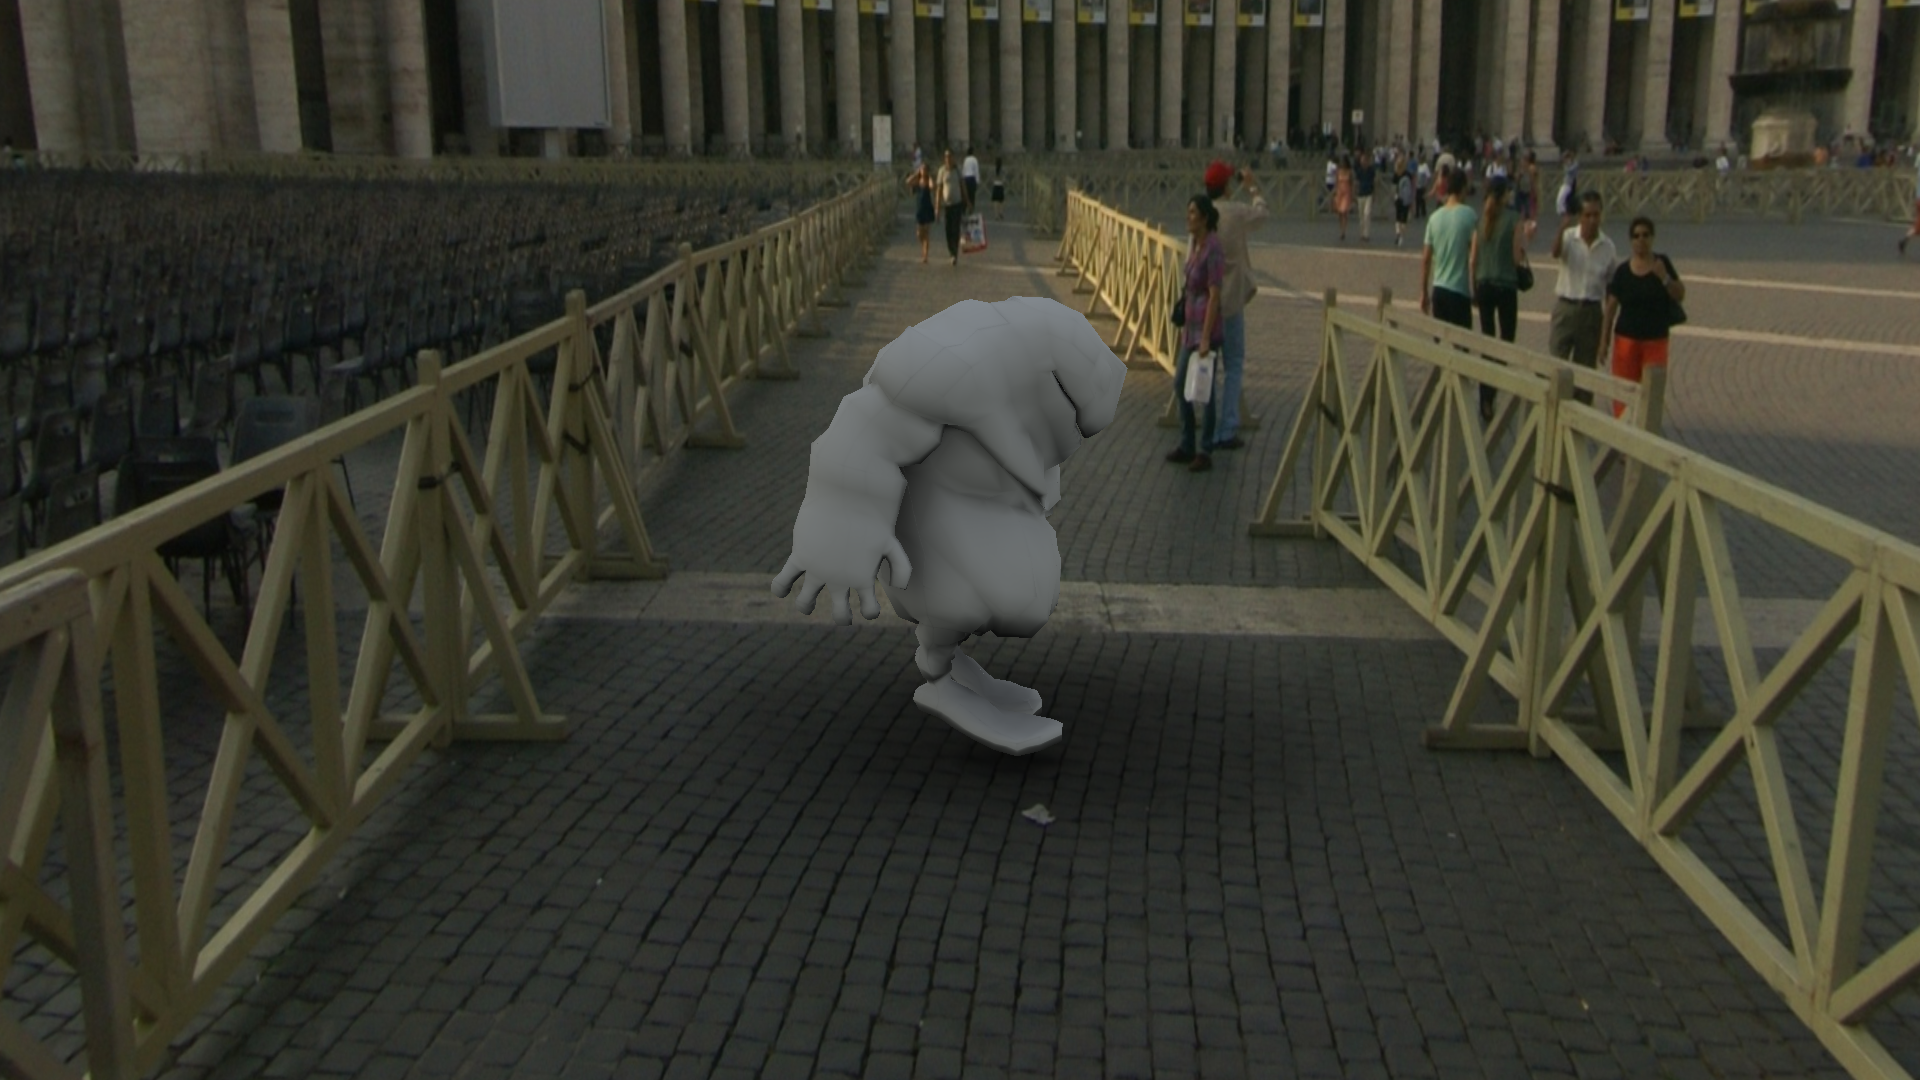
\includegraphics[width=\textwidth]{\rootPath Imgs/screen/white-1.png}
	\end{subfigure}
	\begin{subfigure}[b]{0.3\textwidth}\centering
		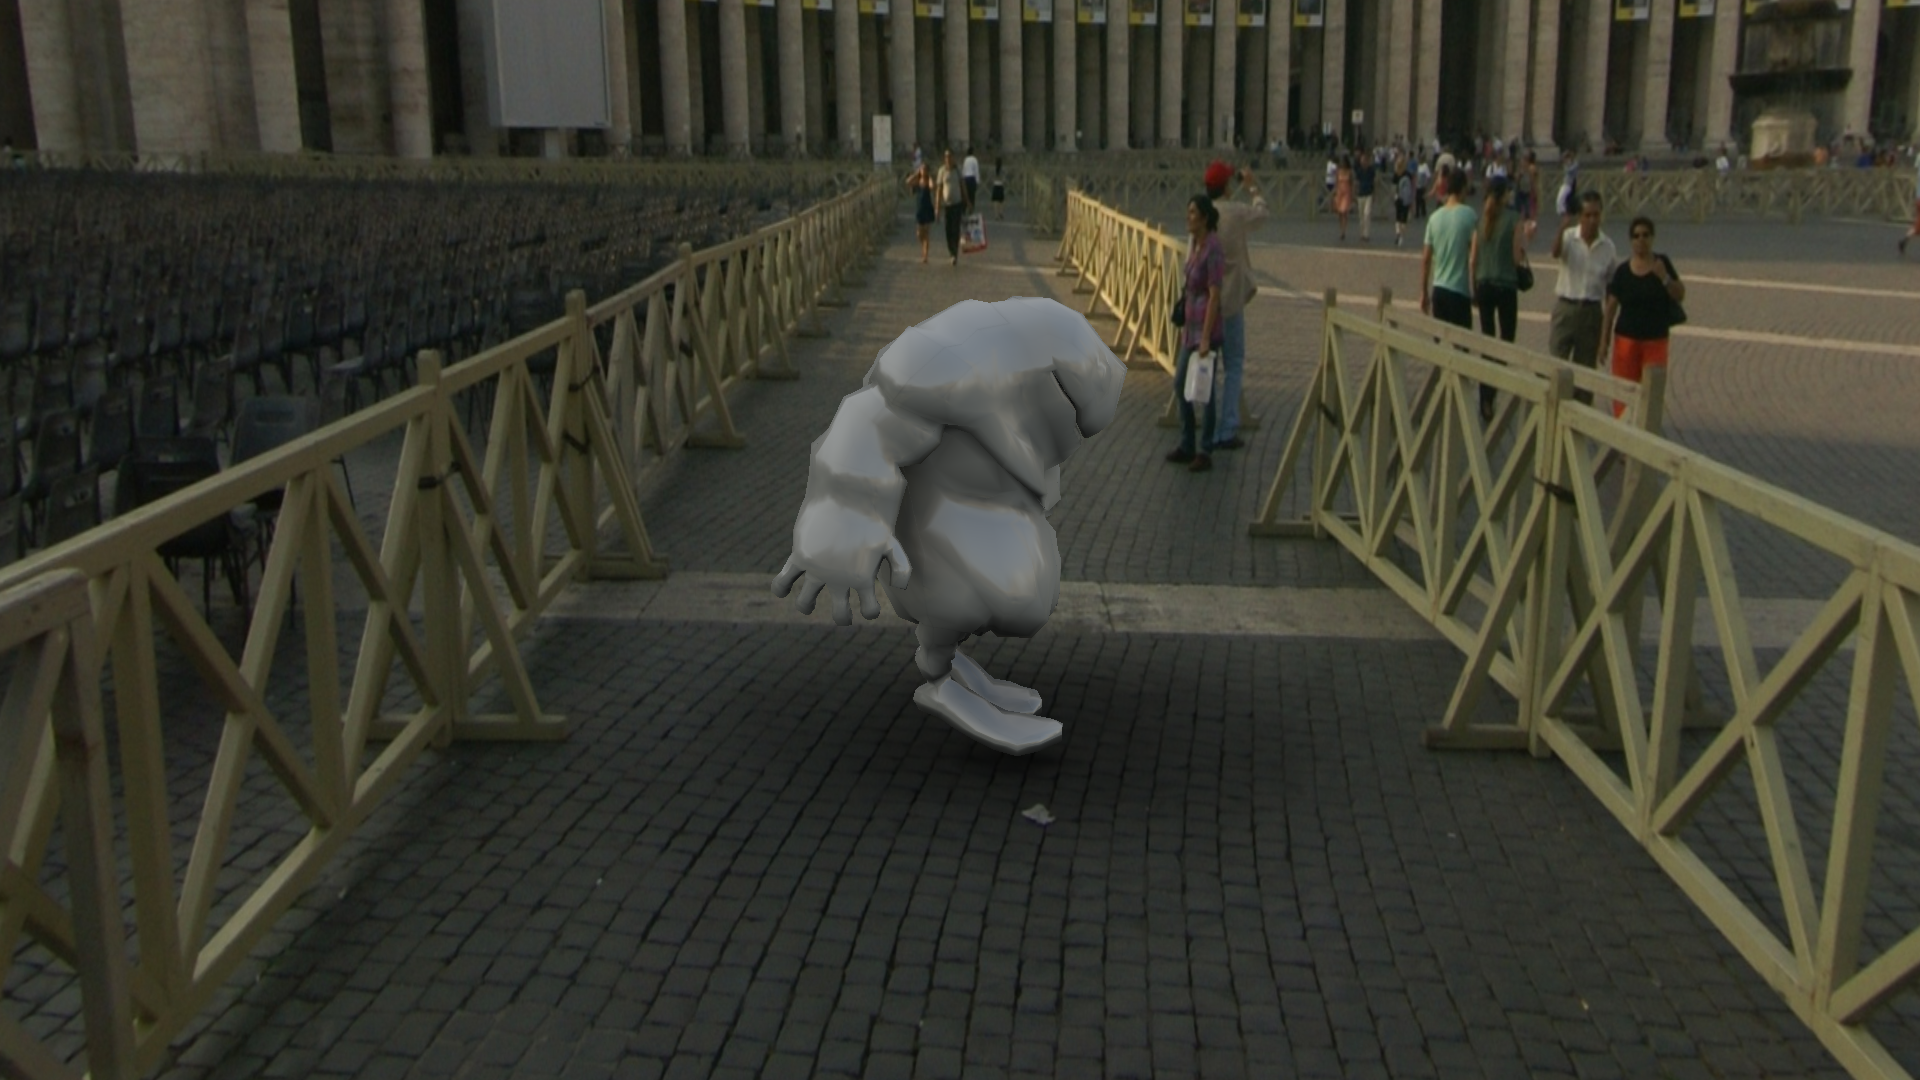
\includegraphics[width=\textwidth]{\rootPath Imgs/screen/glossy-1.png}
	\end{subfigure}
	\begin{subfigure}[b]{0.3\textwidth}\centering
		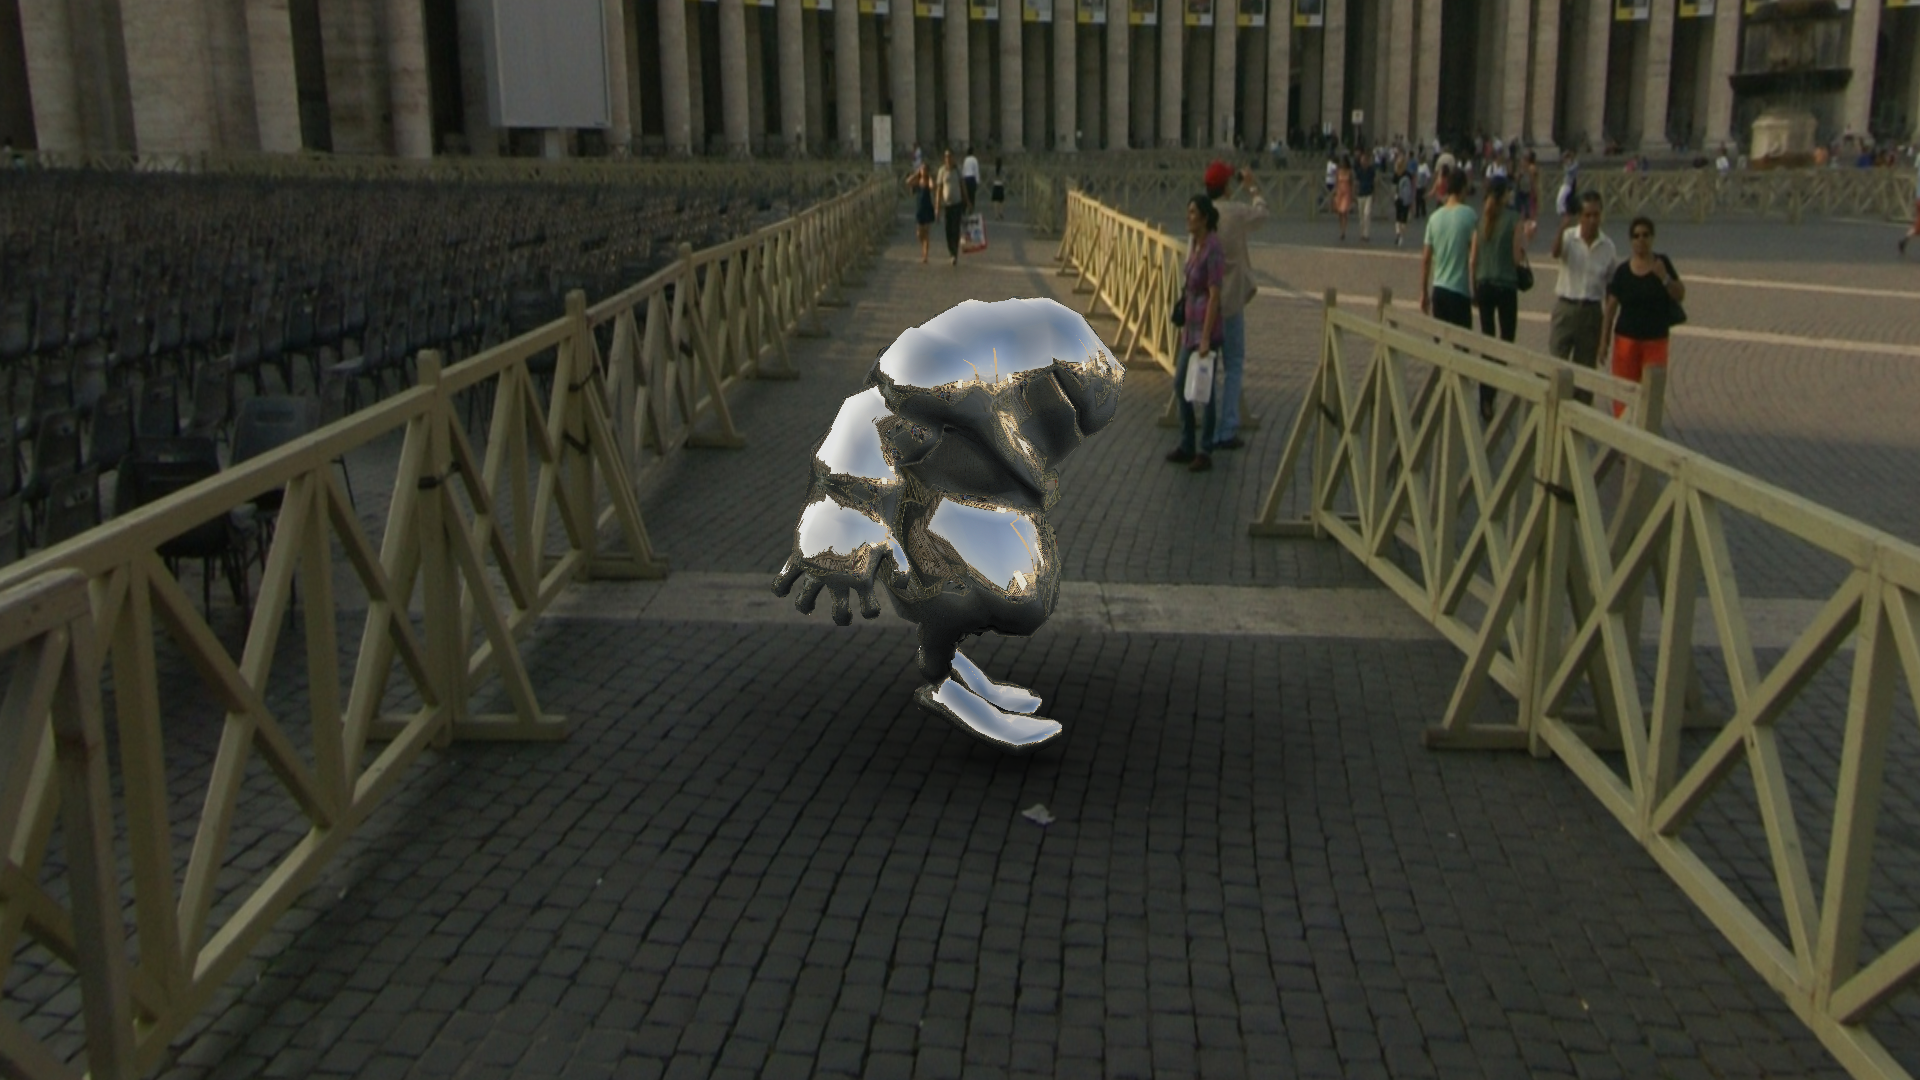
\includegraphics[width=\textwidth]{\rootPath Imgs/screen/miror-1.png}
	\end{subfigure}
	
	\begin{subfigure}[b]{0.3\textwidth}\centering
		\includegraphics[width=\textwidth]{\rootPath Imgs/screen/white-2.png}
	\end{subfigure}
	\begin{subfigure}[b]{0.3\textwidth}\centering
		\includegraphics[width=\textwidth]{\rootPath Imgs/screen/glossy-2.png}
	\end{subfigure}
	\begin{subfigure}[b]{0.3\textwidth}\centering
		\includegraphics[width=\textwidth]{\rootPath Imgs/screen/miror-2.png}
	\end{subfigure}
	
	\begin{subfigure}[b]{0.3\textwidth}\centering
		\includegraphics[width=\textwidth]{\rootPath Imgs/screen/white-3.png}
	\end{subfigure}
	\begin{subfigure}[b]{0.3\textwidth}\centering
		\includegraphics[width=\textwidth]{\rootPath Imgs/screen/glossy-3.png}
	\end{subfigure}
	\begin{subfigure}[b]{0.3\textwidth}\centering
		\includegraphics[width=\textwidth]{\rootPath Imgs/screen/miror-3.png}
	\end{subfigure}
	
	\begin{subfigure}[b]{0.3\textwidth}\centering
		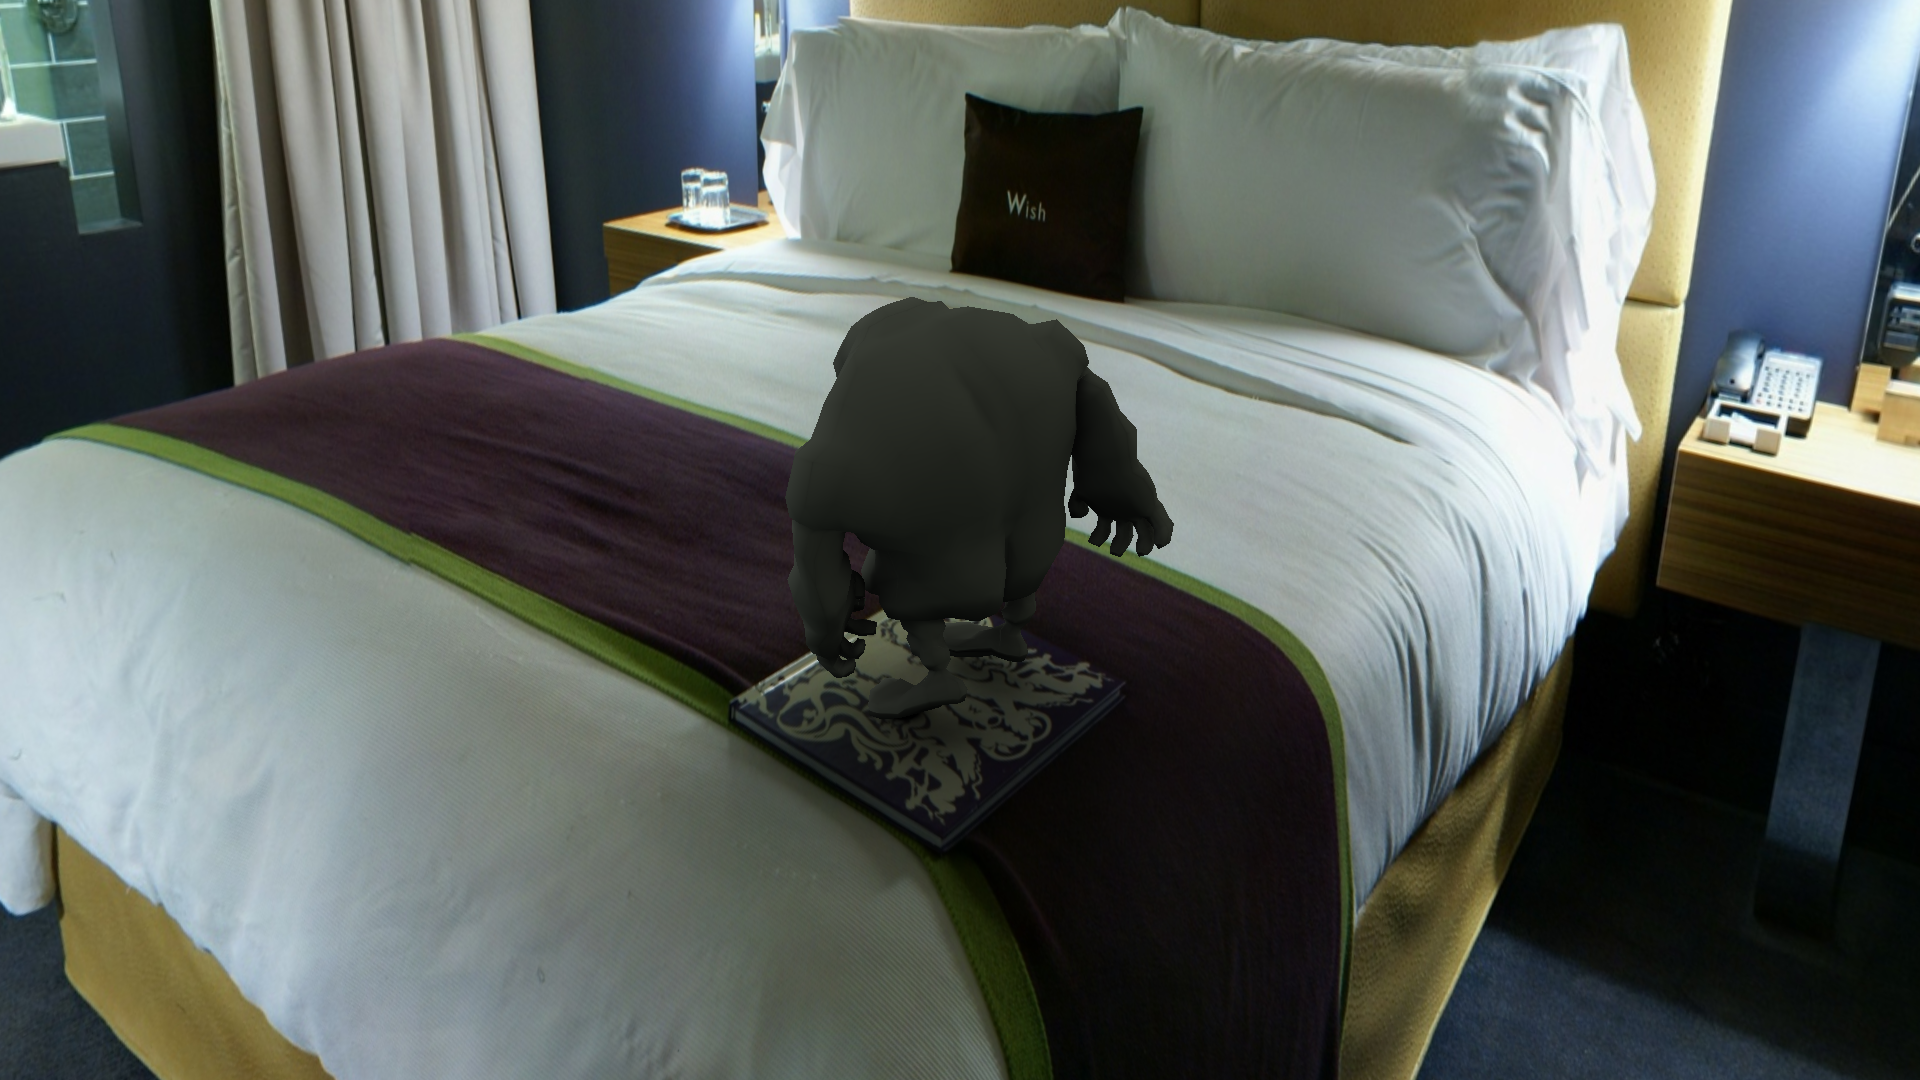
\includegraphics[width=\textwidth]{\rootPath Imgs/screen/white-4.png}
	\end{subfigure}
	\begin{subfigure}[b]{0.3\textwidth}\centering
		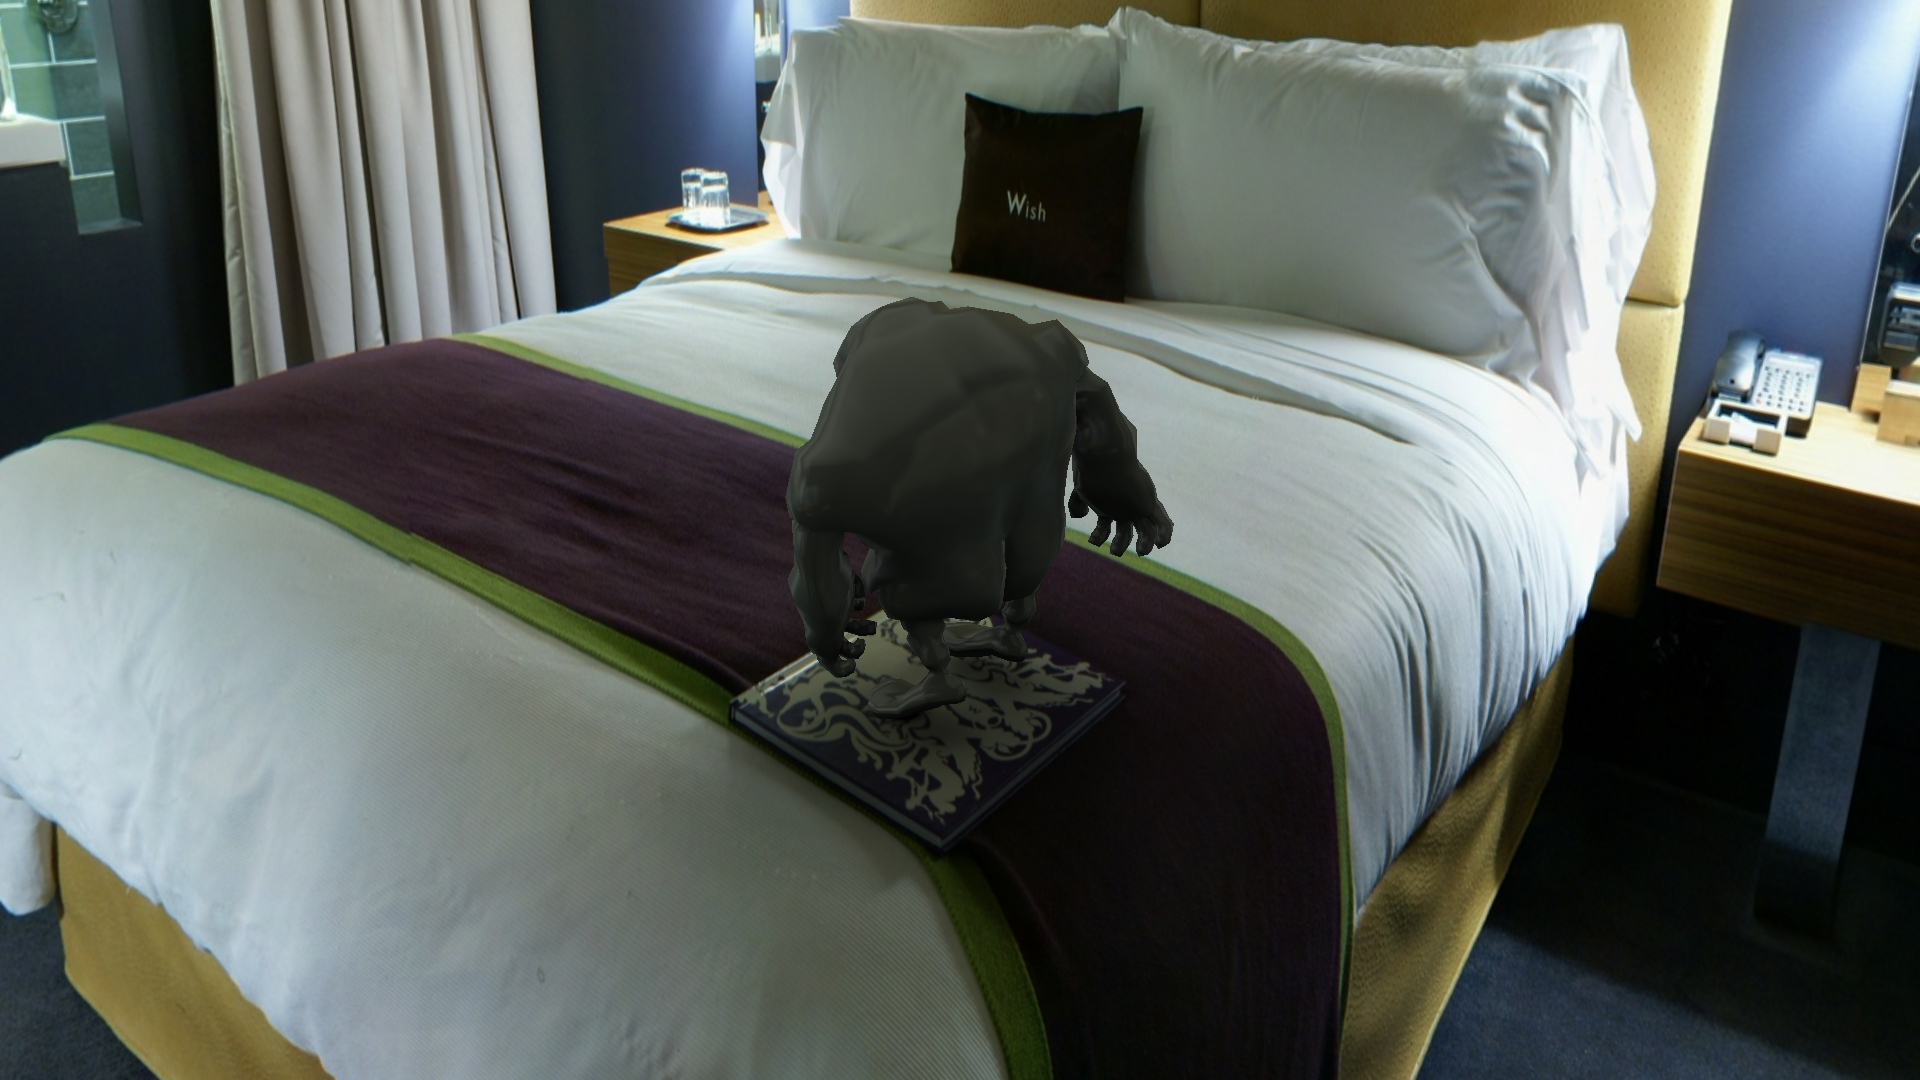
\includegraphics[width=\textwidth]{\rootPath Imgs/screen/glossy-4.png}
	\end{subfigure}
	\begin{subfigure}[b]{0.3\textwidth}\centering
		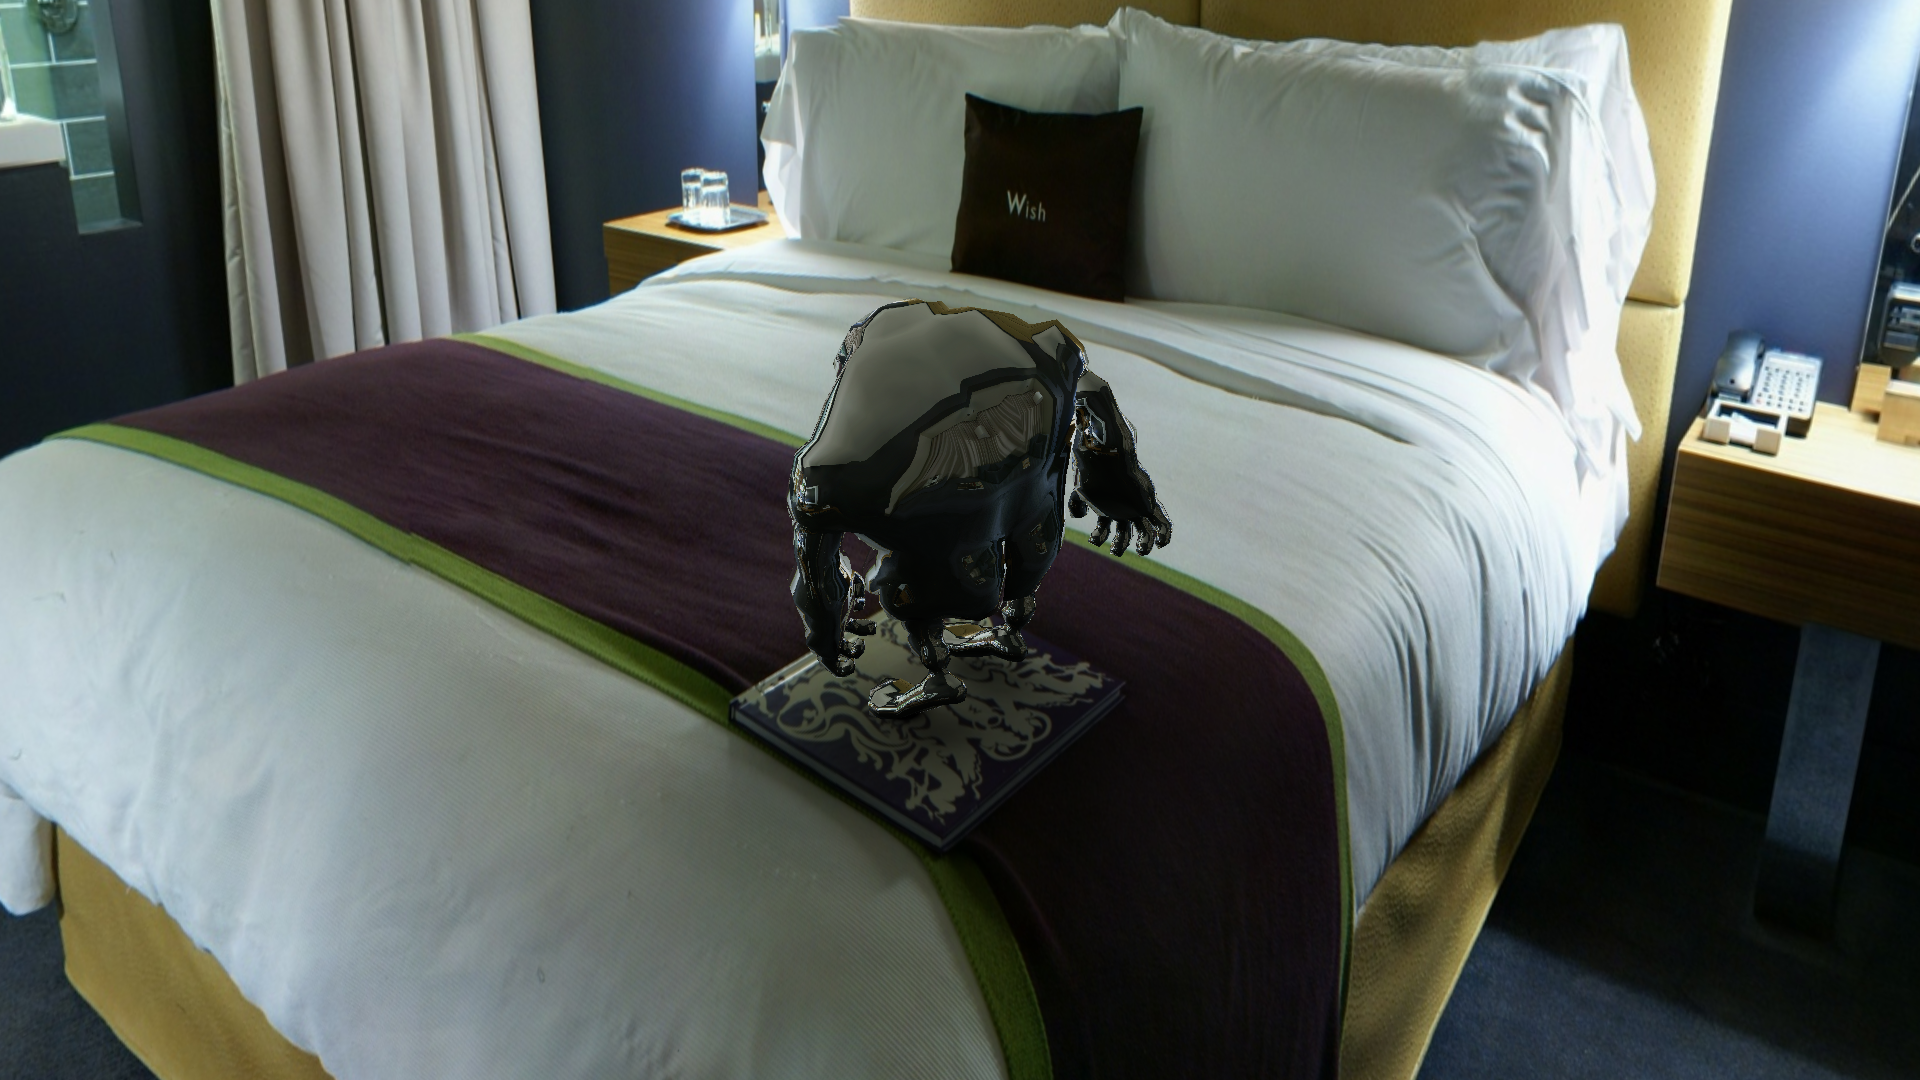
\includegraphics[width=\textwidth]{\rootPath Imgs/screen/miror-4.png}
	\end{subfigure}

	\caption{Rendu du modèle “bigguy” pour differents niveau de spécularité}
	\label{fig:result:specularity}
\end{figure*}


\iftwocolumn \begin{multicols}{2} \fi
L’application développée, ainsi que son portage sur iOS, on permit de valider le modèle de rendu développée au cours de ce stage. À défaut de correspondre aux résultats d’un modèle statistique, les images rendues répondent aux exigences d’intégration vraisemblable. L’aspect temps réel est lui aussi atteint, les performances sur périphérique mobiles allant de $20$ à plus de $60$ images par seconde selon le modèle d’envmap utilisé. Ces performances sont rendu possible grace à l’architecture des terminaux mobiles, le fait que la mémoire CPU et GPU soit partagé reduit en effet le cout des transferts mémoire.

Parallèlement, les mécanismes d’acquisition d’envmap développés permetent l’acquisition des données d’environnements nécessaires à la phase de rendu. Même si de nombreux artefacts sont visibles dans le cas de reflets spéculaires, ils reste invisible pour des matières diffuses. 
\iftwocolumn \end{multicols} \fi


\begin{figure*}[!ht]\centering

	\begin{subfigure}[b]{0.45\textwidth}\centering
		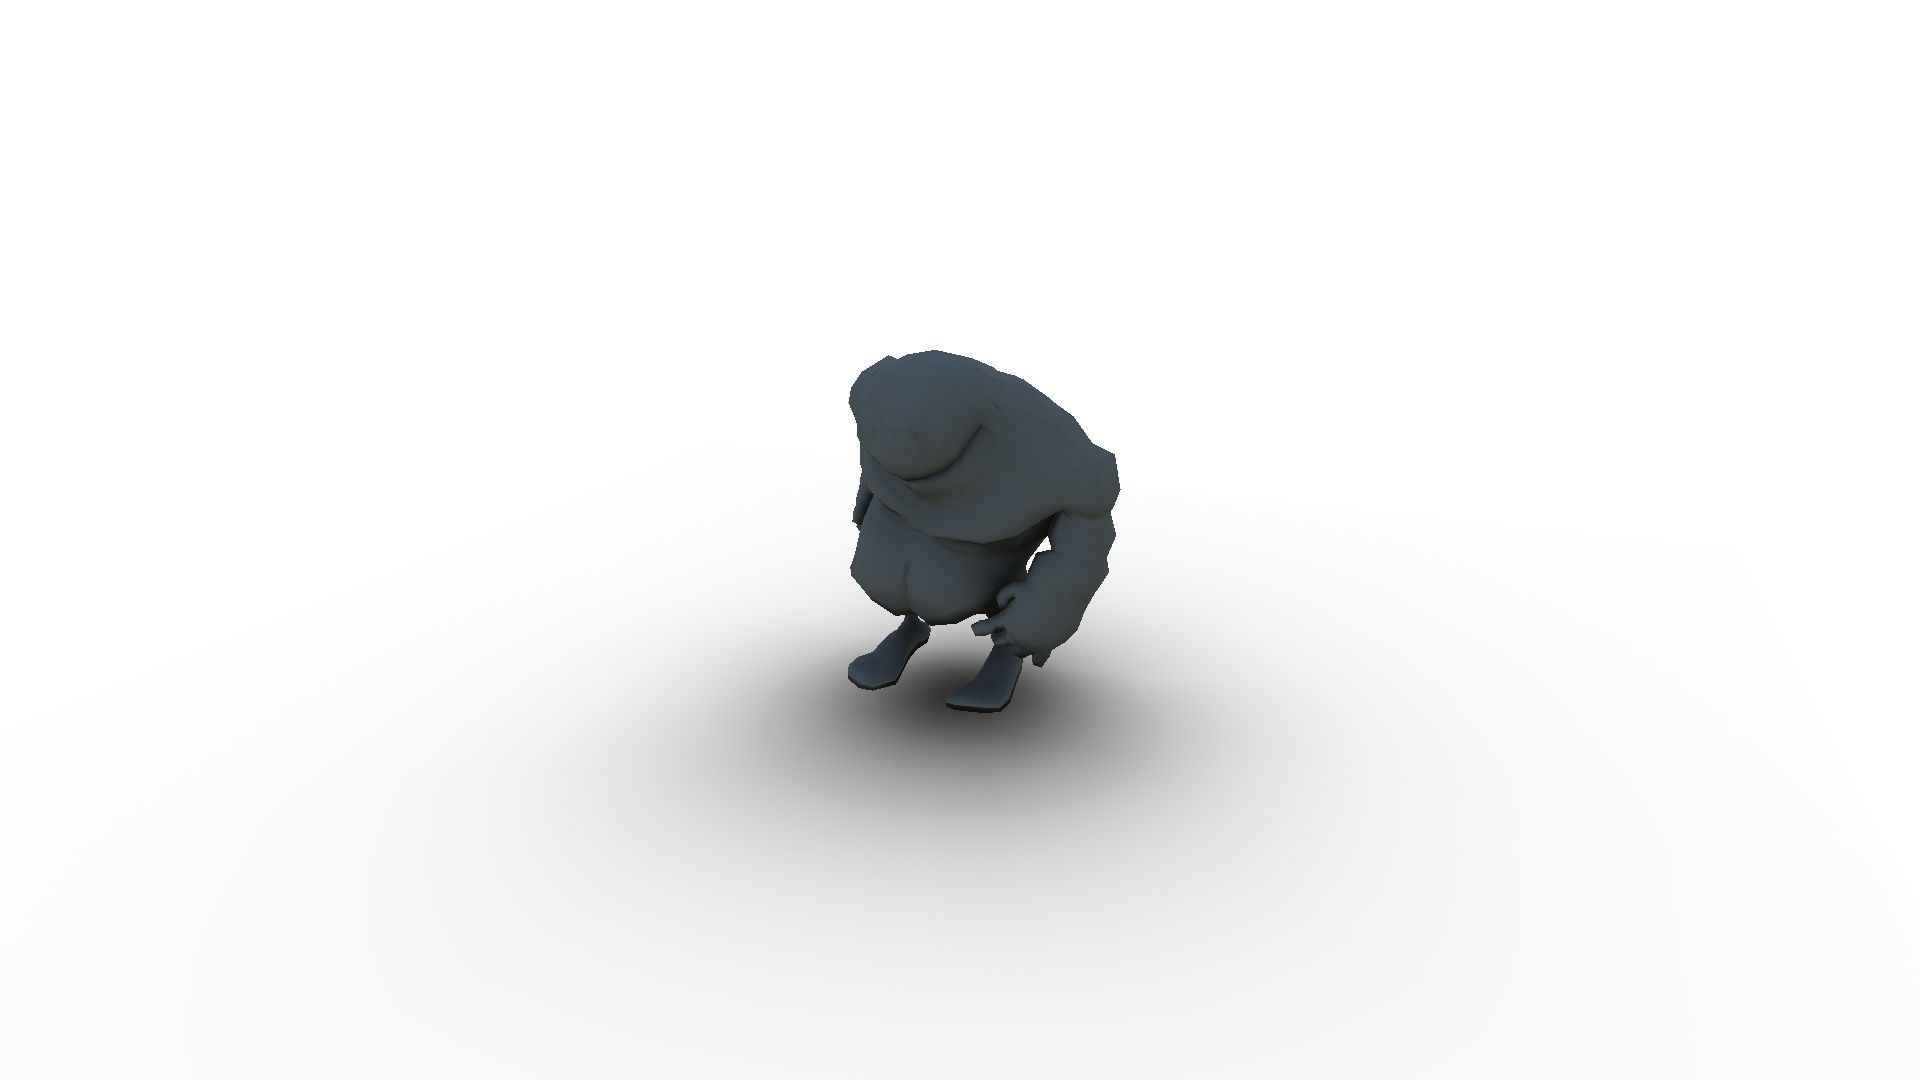
\includegraphics[width=\textwidth]{\rootPath Imgs/screen/sphere-single-1.png}
	\end{subfigure}
	\begin{subfigure}[b]{0.45\textwidth}\centering
		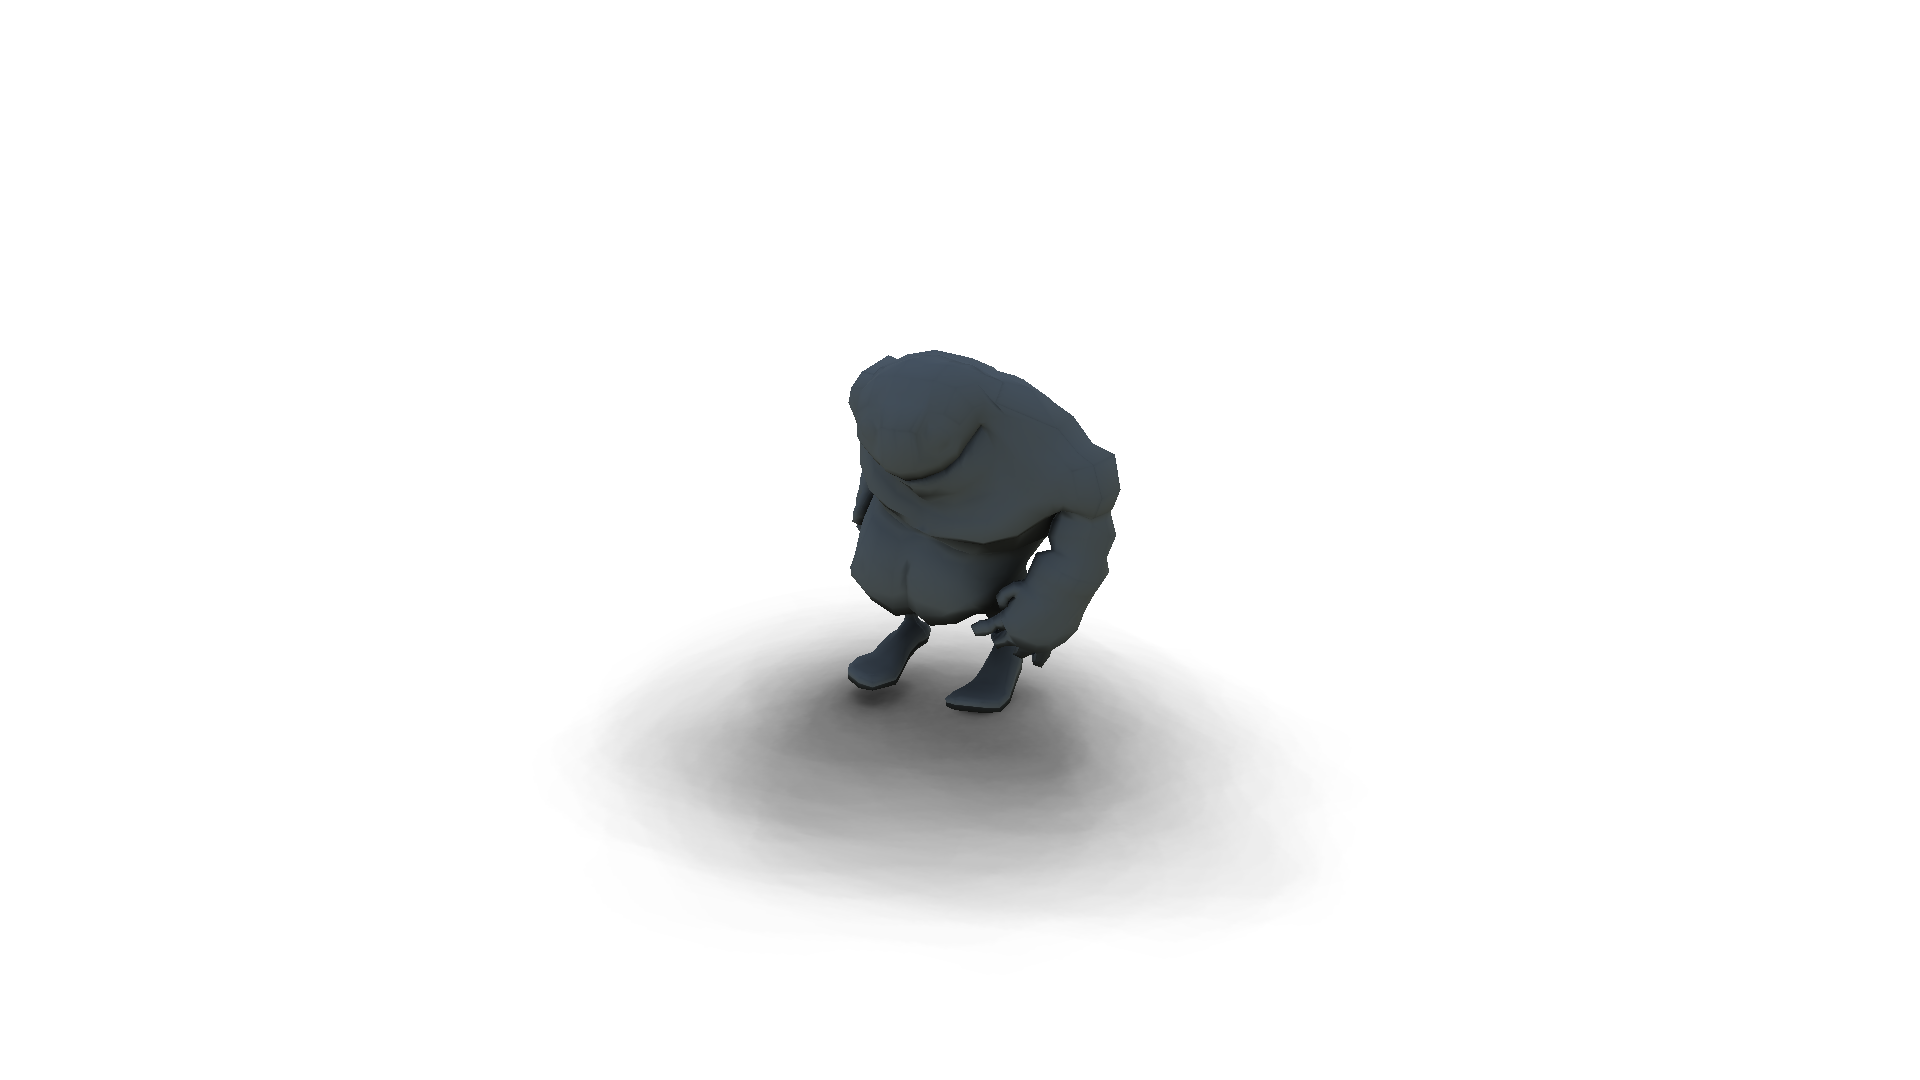
\includegraphics[width=\textwidth]{\rootPath Imgs/screen/sphere-mult-1.png}
	\end{subfigure}
	
	\begin{subfigure}[b]{0.45\textwidth}\centering
		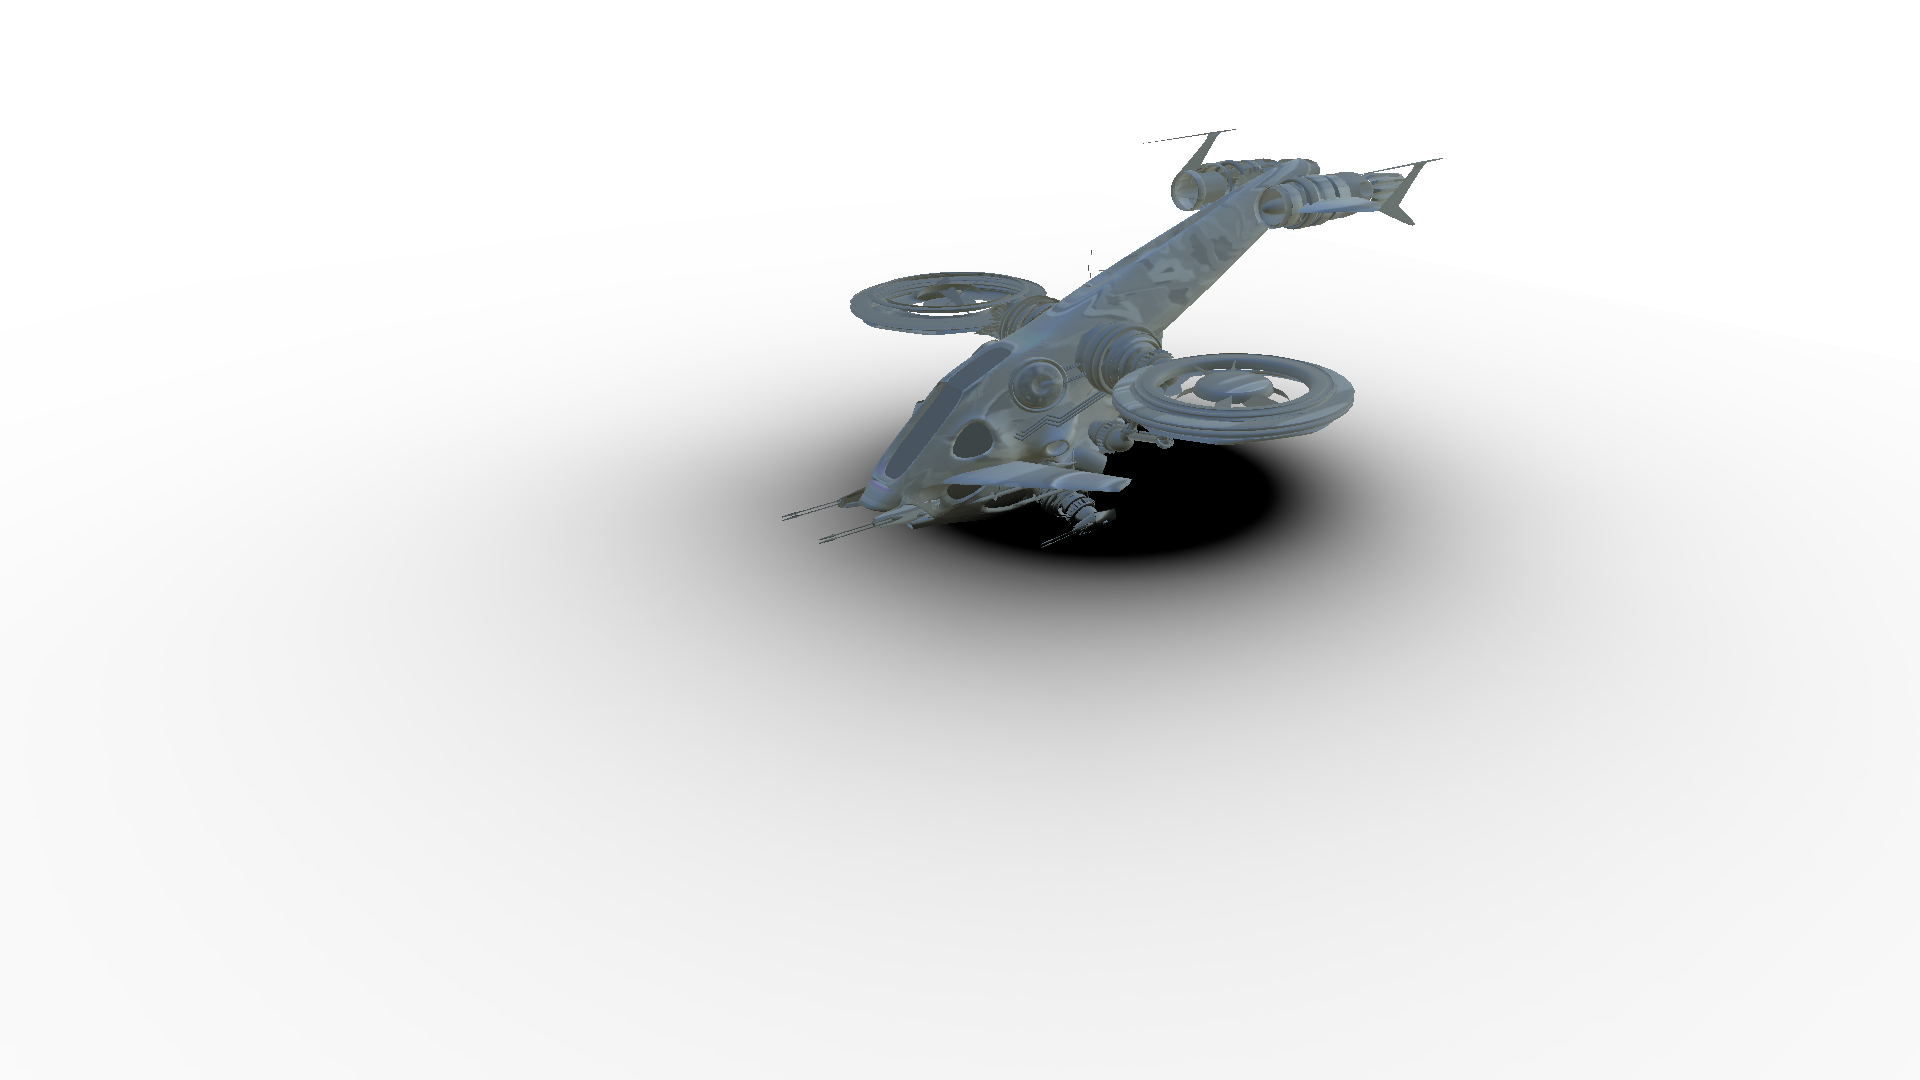
\includegraphics[width=\textwidth]{\rootPath Imgs/screen/sphere-single-2.png}
	\end{subfigure}
	\begin{subfigure}[b]{0.45\textwidth}\centering
		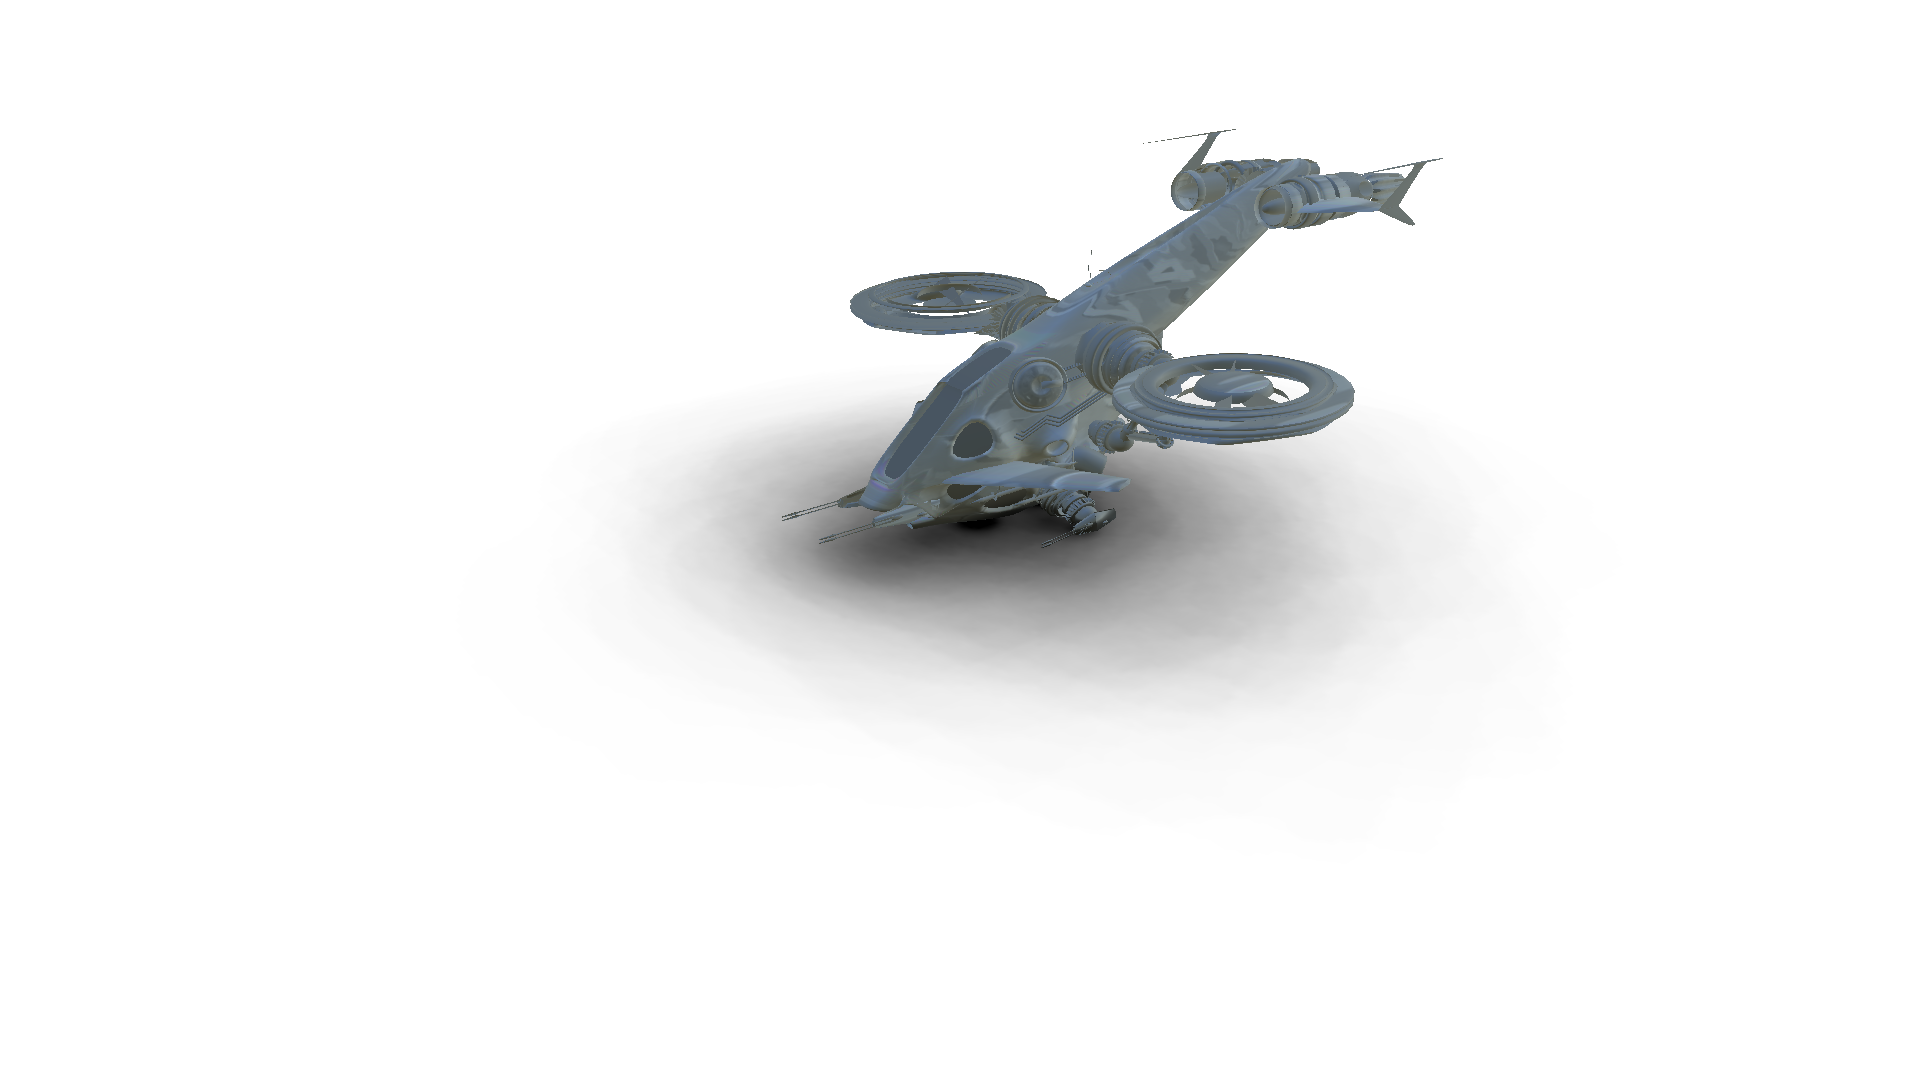
\includegraphics[width=\textwidth]{\rootPath Imgs/screen/sphere-mult-2.png}
	\end{subfigure}
	
	\caption{Rendu des ombres portées sans (gauche) et avec (droite) les informations de sphères englobantes}
	\label{fig:result:spheres}
\end{figure*}


\iftwocolumn \begin{multicols}{2} \fi
Ce portage à permit de confirmer que la génération de terminaux mobiles actuellement sur le marché pressente de fait tous les prérequis, aussi bien matériel que logiciel, nécessaire au développement de la réalité augmentée réaliste et temps réel.

Les méthodes développées sont utilisables de le développement de nombreuses applications mobiles, que ce soit à des fins culturelles (mise en valeur du patrimoine par l’ajout virtuelle d’élément historique) ou à des fins publicitaires (visualisation d’un objet, d’un meuble ou de vêtements avant achat).
\iftwocolumn \end{multicols} \fi


%=====================================================================
%=====================================================================
\ifstandalone
	\addcontentsline{toc}{chapter}{Bibliographie}
	\bibliographystyle{apalike}
	\bibliography{\rootPath Annexes/biblio}
\fi
%=====================================================================
%=====================================================================
\end{document}